\begin{footnotesize}
\begin{frame}
	\frametitle{}
	\maketitle
%	\begin{block}
%	\titlepage
%	\end{block}
\end{frame}

\AtBeginSection[] % Do nothing for \section*
{
	\begin{frame}<beamer>
		\frametitle{Nội dung}
		\tableofcontents[currentsection, currentsubsection]
	\end{frame}
}
%%%%%%%%%%%%%%%%%%%%%%%%
\section{Một số khái niệm}
\subsection{Chuẩn hóa tập mẫu}
\begin{frame}
\frametitle{Chuẩn hóa tập mẫu}
	\begin{itemize}
    \item Chuẩn hóa là một phương pháp tiền xử lý thiết yếu, đặc biệt là trong trường hợp các biến quan sát được đo lường bằng những đơn vị hoặc những thang đo khác nhau (VD: mét, kilogram hay đơn vị tiền tệ). 
    \item Sự khác biệt lớn giữa phạm vi các khoảng giá trị của các biến độc lập có thể tạo ra sự sai lệch trong phân tích để đưa ra một mô hình chính xác. 
    \item VD: Giả sử $z_1$ là biến dự đoán thể hiện chiều cao của một người, vậy thì $z_1 \in [0;2]$ với đơn vị mét. Giả sử $z_2$ là biến dự đoán thể hiện mức chi tiêu của một người (tính theo VNĐ), ta có thể có $z_2 \in [0;10 000 000 000]$. Trong trường hợp hai biến "chiều cao" và "chi tiêu" như trên, "chi tiêu" sẽ có tác động lớn hơn đối với đầu ra (biến phản hồi), nhưng như vậy ta không khẳng định được rằng biến đó có ý nghĩa quan trọng hơn về mặt thống kê. 
\end{itemize}
\end{frame}
%%=====================================
\begin{frame}
\frametitle{Chuẩn hóa tập mẫu}
	\begin{itemize}
	\item Để chuẩn hóa dữ liệu, ta đặt:
   \[
   z^* = \dfrac{z- \mu}{s}
   \]
   Trong đó:
   \begin{itemize}
       \item $z$ là giá trị quan sát
       \item $\mu$ là giá trị trung bình mẫu
       \item $s$ là độ lệch chuẩn
   \end{itemize}
   \item Tác dụng của việc chuẩn hóa dữ liệu:
   \begin{itemize}
       \item Đưa các biến về cùng thang đo.
       \item Tăng độ chính xác và ổn định của mô hình thống kê, tránh việc biến có giá trị lớn chi phối kết quả.
       \item Khi áp dụng công thức này với toàn bộ dữ liệu $Z$, ta sẽ nhận được mẫu $Z^*$ mới có $\mu = 0$ và $s=1$.
   \end{itemize}
	\end{itemize}
\end{frame}
%%=====================================
\subsection{Outlier}
\begin{frame}
\frametitle{Outlier}
	\begin{block}{Định nghĩa}
    \textbf{Outlier} là điểm dữ liệu bất thường, nghĩa là quan sát tại điểm đó khác biệt so với phần còn lại của bộ dữ liệu mà ta thu thập được. 
    \end{block}
    \begin{figure}
        \centering
        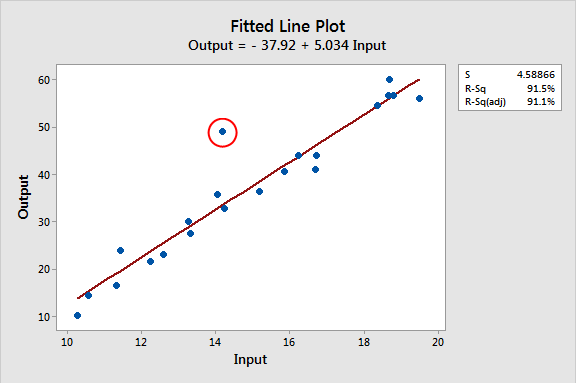
\includegraphics[width=0.55\linewidth]{images/Hình minh họa cho Outlier.png}
        \caption{Hình minh họa cho Outlier}
        \label{fig:placeholder}
    \end{figure}
\end{frame}
%%=====================================
\begin{frame}
\frametitle{Sự tác động của Outlier đến mô hình hồi quy}
	\begin{figure}
	    \centering
	    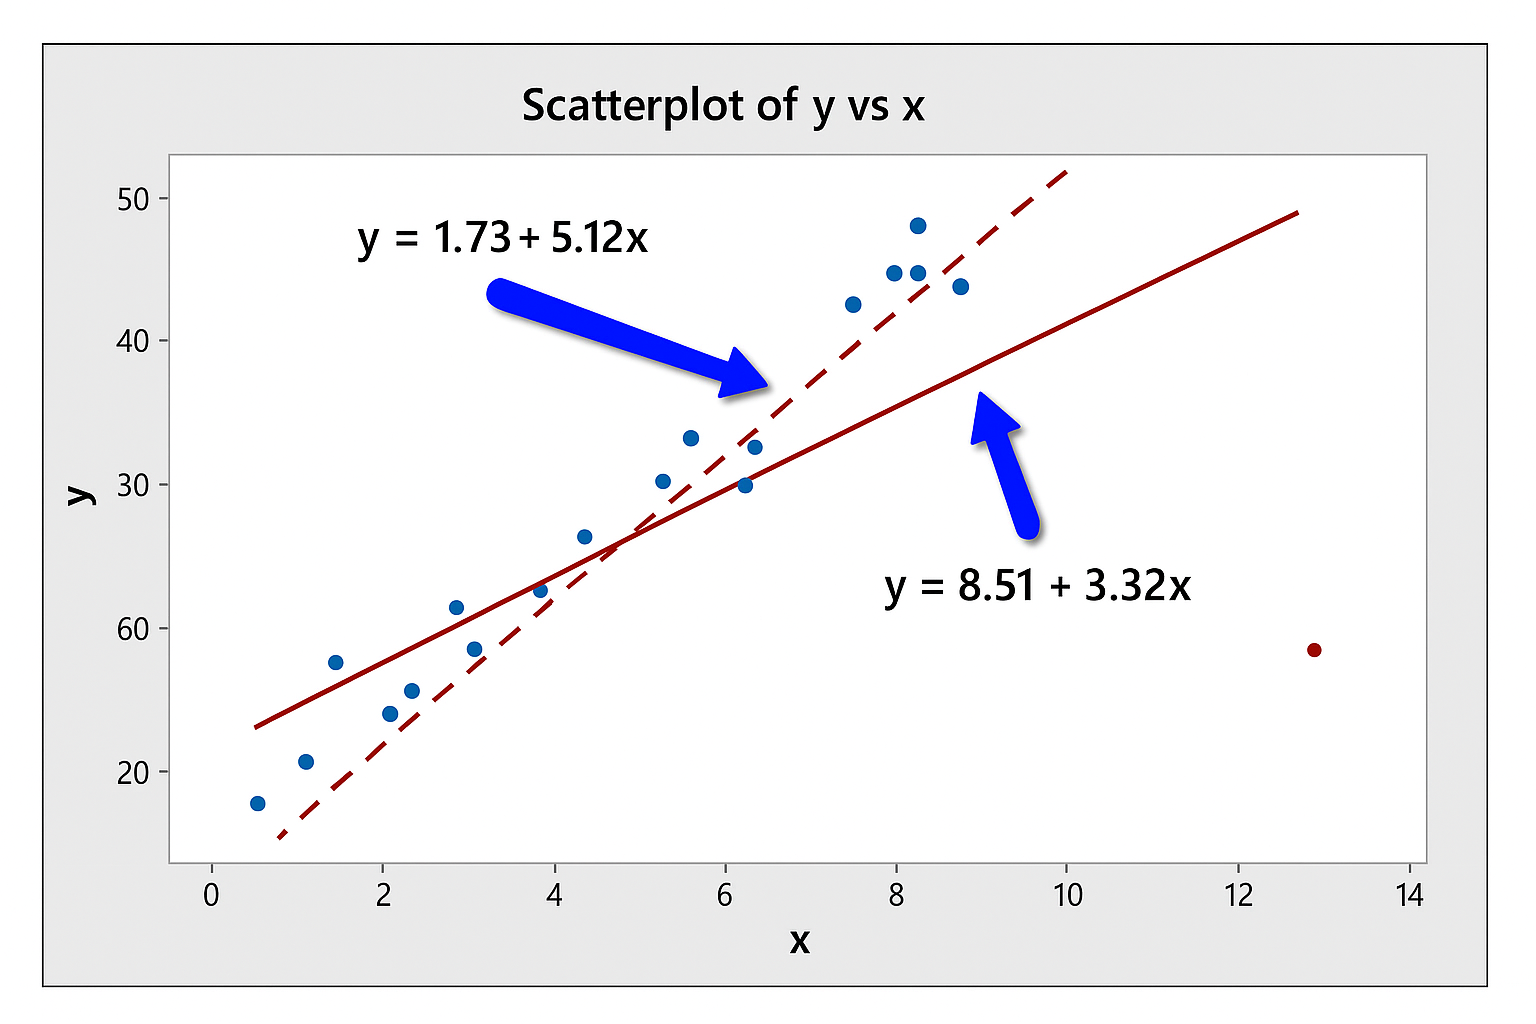
\includegraphics[width=0.6\linewidth]{images/Sự tác động của Outlier đến mô hình.png}
	    \caption{Sự tác động của Outlier đến mô hình}
	    \label{fig:placeholder}
	\end{figure}
    \begin{itemize}
        \item Đường nét liền thể hiện mô hình hồi quy tuyến tính khi giữ lại Outlier.
        \item Đường nét đứt thể hiện mô hình hồi quy tuyến tính khi đã loại bỏ Outlier.
    \end{itemize}
\end{frame}
\subsection{Độ đo Leverage}
\begin{frame}
\frametitle{Độ đo Leverage}
	\begin{itemize}
    \begin{block}{Định nghĩa}
    \textbf{Leverage} là độ đo khoảng cách giữa một điểm dữ liệu và phần còn lại của bộ dữ liệu dựa trên miền giá trị của bộ dữ liệu, được xác định bởi công thức:
    $$ h_{k j}=\frac{1}{n}+\frac{\left(z_{kj}-\overline{z}\right)^{2}}{\sum_{j=1}^{n}\left(z_{kj}-\overline{z}\right)^{2}}$$
    \end{block}
    \item Những điểm nằm xa so với bộ dữ liệu gọi là những điểm high leverage, ngược thì gọi là lower leverage.
    \item \textbf{Kết luận:} Ta thấy $h_{kj}$ luôn nằm giữa 1/n và 1. Hơn nữa, leverage trung bình cho các quan sát luôn bằng (p+1)/n, p là biến số dự đoán. Do vậy, nếu một quan sát mà có độ đo leverage quá lớn so với (p+1)/n ta có thể nghi ngờ là một điểm high leverage.
\end{itemize}
\end{frame}
%%=====================================
\begin{frame}
\frametitle{Nhận xét}
\begin{itemize}
   \item Càng có nhiều điểm dữ liệu nằm gần nhau thì sức ảnh hưởng hay độ lớn của điểm high leverage càng giảm.
   \item Các điểm high leverage có tác động rất lớn đến mô hình, điểm nào có giá trị của biến dự đoán nằm càng xa khỏi bộ dữ liệu thì tác động càng lớn.
   \item Những điểm $h_{kj} > 3*\overline{h}$ thì được coi là những outlier, với $\overline{h} = \dfrac{1}{n}\sum_{j=1}^n{h_{kj}}$
\end{itemize}
\end{frame}
%%=====================================
\begin{frame}
\frametitle{Ví dụ}

Để nghiên cứu sự phụ thuộc giữa điểm thi cuối kỳ $Y$ (tính theo thang 10) và số giờ tự học mỗi tuần $Z_1$, số giờ ngủ trung bình mỗi đêm $Z_2$ (đơn vị giờ), người ta điều tra ngẫu nhiên 12 sinh viên đại học của một trường, thu được bảng số liệu sau:

\resizebox{\textwidth}{!}{%
\begin{tabular}{|c|c|c|}
\hline 
$Y$ (Điểm thi cuối kỳ) & $Z_1$ (Số giờ tự học mỗi tuần) & $Z_2$ (Số giờ ngủ trung bình mỗi đêm) \\
\hline 
5.8 & 6.5 & 6.5 \\
6.5 & 7.0 & 6.0 \\
7.0 & 6.5 & 7.0 \\
7.5 & 8.0 & 6.5 \\
8.0 & 9.0 & 7.2 \\
8.2 & 10.0 & 6.8 \\
7.8 & 8.6 & 7.5 \\
8.8 & 11.0 & 7.0 \\
9.0 & 12.0 & 6.7 \\
6.0 & 6.0 & 6.0 \\
8.3 & 9.5 & 7.8 \\
9.2 & 2.0 & 5.5 \\
\hline
\end{tabular}%
}

\end{frame}

%%=====================================
\begin{frame}
\frametitle{Ví dụ}

Ta có bảng sau:

\resizebox{\textwidth}{!}{%
\begin{tabular}{|c|ccc|c|ccc|}
\hline 
$j$ & $z_1$ & $h_{1j}$ & $h_{1 j} > 3*\frac{1}{n}\sum_{j=1}^{n}{h_{1 j}}$ 
& $j$ & $z_2$ & $h_{2j}$ & $h_{2 j} > 3*\frac{1}{n}\sum_{j=1}^{n}{h_{2 j}}$ \\
\hline
1 & 6.5 & 0.1125 & 0 & 1 & 6.5 & 0.0924 & 0 \\
2 & 7.0 & 0.0964 & 0 & 2 & 6.0 & 0.1881 & 0 \\
3 & 6.5 & 0.1125 & 0 & 3 & 7.0 & 0.1011 & 0 \\
4 & 8.0 & 0.0833 & 0 & 4 & 6.5 & 0.0924 & 0 \\
5 & 9.0 & 0.0959 & 0 & 5 & 7.2 & 0.1338 & 0 \\
6 & 10.0 & 0.1341 & 0 & 6 & 6.8 & 0.0851 & 0 \\
7 & 8.6 & 0.0878 & 0 & 7 & 7.5 & 0.2142 & 0 \\
8 & 11.0 & 0.1979 & 0 & 8 & 7.0 & 0.1011 & 0 \\
9 & 12.0 & 0.2873 & 0 & 9 & 6.7 & 0.0833 & 0 \\
10 & 6.0 & 0.1350 & 0 & 10 & 6.0 & 0.1881 & 0 \\
11 & 9.5 & 0.1118 & 0 & 11 & 7.8 & 0.3322 & 0 \\
12 & 2.0 & 0.5455 & 1 & 12 & 5.5 & 4.7122 & 1 \\
\hline
\end{tabular}%
}

\vspace{0.5em}
Trong bộ dữ liệu ở ví dụ 6.1, quan sát thứ 12 ($Y=9.2$, $z_1 = 2.0$, $z_2 = 5.5$) là một \textbf{outlier} vì điểm này có kết quả thi rất cao mặc dù thời gian học và ngủ thấp, trái ngược với xu hướng chung.
\end{frame}

%%======================
%%=====================================
\subsection{Quy tắc 1.5IQR}
\begin{frame}
\frametitle{Quy tắc 1.5IQR}
\begin{itemize}
    \item Bất kì tập dữ liệu nào cũng có thể mô tả bằng năm giá trị đặc trưng, năm giá trị này cung cấp thông tin cần thiết để định vị outlier bao gồm (lần lượt theo thứ tự tăng dần).
    \begin{itemize}
        \item Giá trị nhỏ nhất hoặc thấp nhất của tập dữ liệu.
        \item Tứ phân vị thứ nhất $Q_1$: Phân vị mức 25\%.
        \item Tứ phân vị thứ hai $Q_2$: Phân vị mức 50\%.
        \item Tứ phân vị thứ ba $Q_3$: Phân vị mức 75\%.
        \item Giá trị lớn nhất hoặc cao nhất của tập dữ liệu.
    \end{itemize}
    \item \textbf{Khoảng cách tứ phân vị} là giá trị
    \[
    IQR = Q_3 - Q_1
    \]
    Khi đó nếu $x \notin \left[Q_1 - 1.5IQR, Q_3 + 1.5IQR\right]$ thì $x$ sẽ được coi là một điểm outlier.
\end{itemize}
\end{frame}
%%=====================================
%%=====================================
\begin{frame}
\frametitle{Ví dụ}
	    Một hệ thống ghi lại tốc độ (đơn vị: km/h) của 25 xe qua trạm như sau: 
        \begin{center}
            \begin{tabular}{|c|c|c|c|c|c|c|c|c|c|c|c|c|}
	\hline 
	20 & 41 & 41 & 80 & 40 & 52 & 52 & 52 & 60 & 55 & 60 & 60 & 62 \\ \hline
60 & 55 & 60 & 55 & 92 & 70 & 35 & 40 & 30 & 30 & 80 & 25 &  \\ \hline
\end{tabular}
        \end{center}
        Tìm các số liệu bất thường (nếu có) trong mẫu số liệu trên.
\end{frame}
%%=====================================
\begin{frame}
\frametitle{Ví dụ}
\begin{itemize}
	\item Sắp xếp dữ liệu theo thứ tự tăng dần: 20, 25, 30, 30, 35, 40, 40, 41, 41, 52, 52, 52, 55, 55,  60, 60, 60, 60, 60, 62, 70, 80, 80, 92.
    \item $Q_1$ là trung bình cộng giá trị thứ 6 và 7 nên $Q_1 = \dfrac{40 + 40}{2} = 40$.
    \item $Q_3$ là trung bình cộng giá trị thứ 19 và 20 nên $Q_3 = \dfrac{60 + 60}{2} = 60$.
    \item $IQR = Q_3 - Q_1 = 60 - 40 = 20$.
    \item Giới hạn dưới: $Lower = Q_1 - 1.5IQR = 40 - 1.5*20 = 40 - 30 = 10$.
    \item Giới hạn trên: $Upper = Q_3 + 1.5IQR = 60 + 1.5*20 = 60 + 30 =  90$.
\end{itemize}
\textbf{Kết luận}: Trong tập dữ liệu này, giá trị 92 là một outlier vì nó nằm ngoài khoảng $(Lower, Upper) = (10,90)$
\end{frame}
%%=====================================
\begin{frame}
\frametitle{Nhận xét}
Quy tắc \textit{1.5IQR} loại bỏ outlier được bắt nguồn từ quy tắc $3 \sigma$ trong lý thuyết xác suất. Quy tắc này phát biểu như sau:\textit{"Gần như chắc chắn rằng (với độ tin cậy khoảng 99,73\%) biến ngẫu nhiên $X$ có phân phối chuẩn} $\mathcal{N}(\mu, \sigma^2)$ \textit{sẽ lấy giá trị trong khoảng lân cận $3 \sigma$ của giá trị trung bình $\mu$"}. 
Với quy tắc này, ta có thể coi các giá trị nằm ngoài khoảng $(\mu - 3\sigma, \mu+3\sigma)$ là outlier. Tuy nghiên trên thực tế, khoảng $\left[Q_1-1.5IQR;Q_3+1.5IQR\right]$ chưa lấy được hết lân cận $3 \sigma$ mà chỉ lấy được tới lân cận $2.7 \sigma$ của giá trị trung bình $\mu$.
Do đó nếu cần thiết, ta có thể hiệu chỉnh quy tắc này trở thành quy tắc $1.7IQR$ để có thể lấy được hết lân cận, khi đó, nếu $x \notin \left[Q_1-1.7IQR; Q_3+1.7IQR\right]$ thì $x$ được coi là một điểm outlier.
\end{frame}
%%============================
\subsection{Giá trị $t-$statistic và $p-$value}
\begin{frame}
\frametitle{Định nghĩa $p-$value và $t-$statistic}
\begin{block}{Định nghĩa}
\begin{itemize}
   \item \textbf{$p-$value} là giá trị có ý nghĩa biên của một kiểm định giả thuyết thống kê, đại diện cho xác suất xảy ra một sự kiện cụ thể, dùng để đánh giá tính đáng tin cậy của một kết quả thống kê và quyết định liệu ta có đủ bằng chứng thống kê để bác bỏ giả thuyết không hay không.
   \item \textbf{$t-$statistic} là đại lượng kiểm định dùng để đánh giá xem một hệ số hồi quy $\beta_i$ có khác không một cách có ý nghĩa thống kê hay không, bằng cách chuẩn hóa $\widehat{\beta_i}$ theo độ lệch chuẩn của nó.
\end{itemize}
\end{block}
\end{frame}
%%=====================================
\begin{frame}
\frametitle{Tìm giá trị $t-$statistic và $p-$value}
   Xét cặp giả thuyết và đối thuyết sau với mỗi $i=\overline{1,r}$.
   \[
   H_0: \beta_i = 0, H_1: \beta_i \ne 0  
   \]
   Việc bác bỏ hay chấp nhận giả thuyết $H_0$ được thực hiện thông qua giá trị $t-$statistic được xác định bởi công thức:
       \[
       t-statistic(Z_i) = \dfrac{\widehat{\beta_i}}{\sqrt{\widehat{D}\left(\widehat{\beta_i}\right)}}
       \]
       Trong đó:
      \begin{itemize}
           \item $\widehat{\beta_i}$ là ước lượng hệ số hồi quy.
           \item $\widehat{D}\left(\widehat{\beta_i}\right)$ là phần tử thứ $i+1$ trên đường chéo chính của ma trận $\widehat{\sigma}^2\left(Z'Z\right)^{-1}$ với $\widehat{\sigma}^2 = \dfrac{1}{n-r-1}\sum_{j=1}^{n}{\widehat{\varepsilon_j}}^2$
       \end{itemize}
       
\end{frame}
%%=====================================
\begin{frame}
\frametitle{Tìm giá trị $t-$statistic và $p-$value}
Giá trị $p-$value là xác suất xảy ra sai lầm loại I (bác bỏ giả thuyết $H_0$ khi $H_0$ đúng)
\[
p-value \left(Z_i\right) = 2 \left(1-CDF(n,|t-statistic(Z_i|)\right)
\]
Trong đó: CDF là hàm phân phối xác suất của phân phối Student.
\end{frame}
%%=====================================
\begin{frame}
\begin{block}{Hệ quả}
\frametitle{Hệ quả}
\begin{itemize}
\item Nếu có mối quan hệ giữa $Z_i$ và $Y$, ta kỳ vọng $t-$statistic có phân phối Student với $n-r-1$ bậc tự do.
\item Giả thuyết $H_0: \beta_i = 0$ bị bác bỏ khi $p-$value < 5\% hoặc $p-$value < 1\% tùy mức ý nghĩa mà ta chọn (thường là 5\%)
\item Khi $ n \ge 30$, chúng lần lượt tương ứng với $t-$statistic $\ge 2$ hoặc $t-$statistic $\ge 2.75$.
\end{itemize}
\end{block}
\end{frame}
%%=====================================
\section{Kiểm định tính phụ thuộc vào biến của mô hình}
\subsection{Kiểm định F về ý nghĩa cùa mô hình hồi quy}
\begin{frame}
\frametitle{Kiểm định F về ý nghĩa của mô hình hồi quy}
Để kiểm định xem liệu trong số các biến $Z_1,Z_2,...,Z_k$ có biến nào là có thể loại khỏi mô hình hồi quy tuyến tính bội, ta tiến hành $F$-test. Việc này được tiến hành bằng cách giả sử rằng một vài hệ số $\beta_k$ của chúng ta bằng 0 (đồng nghĩa với việc loại bỏ $Z_k$) hay ta xét cặp giả thiết và đối thuyết như sau:
\begin{itemize}
    \item Giả thuyết $H_0$: $\beta_1$ =  $\beta_2$ = ... =  $\beta_k$ = 0
    \item Đối thuyết $H_1$: $\exists\beta_j \neq 0$ với j= $\overline{1,k}$ 
\end{itemize}

Tính toán đại lượng $F - score$:
\begin{equation*}
	F = \dfrac{(n-k-1)R^2}{k(1-R^2)}
\end{equation*}

Trong đó:
\[
R^{2} := 
\dfrac{\widehat{y}'\,\widehat{y} - n\bar{y}^{2}}
      {y'\,y - n\bar{y}^{2}}
= 
\dfrac{\displaystyle\sum_{i=1}^{n} (\widehat{y}_{i} - \bar{y})^{2}}
      {\displaystyle\sum_{i=1}^{n} (y_{i} - \bar{y})^{2}}
= 
1 - 
\dfrac{\displaystyle\sum_{i=1}^{n} \widehat{\varepsilon}_{i}^{2}}
      {\displaystyle\sum_{i=1}^{n} (y_{i} - \bar{y})^{2}}
\] 
\end{frame}
%%=====================================
\subsection{Các bước kiểm tra}
\begin{frame}
\frametitle{Các bước kiểm tra}
\begin{itemize}
 \item Bước 1: Tính đại lượng F-score.
    \item Bước 2: Tra bảng phân phối Fisher với bậc tự do là $k$ và $n-k-1$, mức ý nghĩa $\alpha$.
    \item Bước 3: Nếu $F > F_{k,n-k-1}(\alpha)$ thì ta bác bỏ $H_0$ và chấp nhận $H_1$.
\end{itemize}
\end{frame}
%%=====================================
\begin{frame}
\frametitle{Ví dụ}
 Để nghiên cứu sự phụ thuộc giữa doanh thu với chi phí sản xuất và chi phí tiếp thị (đơn vị Dollar), người ta điều
 tra ngẫu nhiên doanh thu của 12 công ty trong 12 thời kỳ, kết quả ta có bảng sau:
     {\scriptsize\begin{center}
            \begin{tabular}{|c|c|c|c|}
	\hline 
	STT & Y (Doanh thu) & $Z_1$ (Chi phí sản xuất) & $Z_2$ (Chi phí tiếp thị) \\
	\hline 
	1& 127 & 18 & 10 \\
      2&  149 & 25 & 11 \\
        3&106 & 19 &6\\
        4&163 & 24 &16\\
        5&102 & 15 &7\\
        6&180 &26 &17\\
        7&161 &25 &14\\
        8&128 &16 &12\\
        9&139 &17 &12\\
        10&144 &23 &12\\
        11&159 &22 &14\\
        12&138 &15 &15\\
	\hline
        
	   \end{tabular}
        \end{center}}
        Ta đi sẽ kiểm tra xem mô hình có phụ thuộc vào biến hay không với $\alpha = 0,05$.
\end{frame}
%%=====================================
\begin{frame}
\frametitle{Ví dụ}
Xét mô hình hồi quy tuyến tính cổ điển, ta có: 
\[
y_i = \beta_0 + \beta_1z_{j1} + \beta_2z_{j2} + \varepsilon_j (j=\overline{1,12}).
\]
Từ bảng trên ta có:\\
\[
Z = \begin{bmatrix}
1 & 18 & 10 \\
1 & 25 & 11 \\
1 & 19 & 6 \\
1 & 24 & 16 \\
1 & 15 & 7 \\
1 & 26 & 17 \\
1 & 25 & 14 \\
1 & 16 & 12 \\
1 & 17 & 12 \\
1 & 23 & 12 \\
1 & 22 & 14 \\
1 & 15 & 15
\end{bmatrix}, y = \begin{bmatrix}
    127 \\ 149 \\ 106 \\ 163\\ 102 \\ 180\\ 161\\128\\139\\144\\159\\138
\end{bmatrix}
\]
\end{frame}
%%=====================================
\begin{frame}
\frametitle{Ví dụ}
Bằng phương pháp ước lượng bình phương cực tiểu, ta tín hđược giá trị ước lượng của các hệ số hồi quy
 như sau:\\
 \[
 \widehat{\beta} = (Z'Z)^{-1}Z'y = \begin{bmatrix}
     \dfrac{1422007}{44056}\\[0,5cm] \dfrac{275981}{110140}\\[0,5cm] \dfrac{209649}{44056}
 \end{bmatrix}
 \]
 Từ đây ta tính được phương trình hồi quy tuyến tính mẫu là:
 \[
 \widehat{y} = \dfrac{1422007}{44056} + \dfrac{275981}{110140}z_1 + \dfrac{209649}{44056}z_2.
 \]
 Suy ra sai số ước lượng của mô hình hồi quy tuyến tính được tính như sau: 
 \[
 \widehat{\varepsilon} = y - Z\widehat{\beta}
 \]
\end{frame}
%%=====================================
\begin{frame}
\frametitle{Ví dụ}
Bảng tính các giá trị $\widehat{y_j}, \widehat{\varepsilon_j}$: 
\begin{center}
    \begin{tabular}{|c|c|c|c|}
    \hline 
    STT & $y_j$ & $\widehat{y_j}$ & $\widehat{\varepsilon_j}$ \\
    \hline 
    1  & 127 & 124.9673 & 2.0327 \\
    2  & 149 & 147.2661 & 1.7339 \\
    3  & 106 & 108.4383 & -2.4383 \\
    4  & 163 & 168.5539 & -5.5539 \\
    5  & 102 & 103.1741 & -1.1741 \\
    6  & 180 & 178.3240 & 1.6760 \\
    7  & 161 & 161.5422 & -0.5422 \\
    8  & 128 & 129.4732 & -1.4732 \\
    9  & 139 & 131.9790 & 7.0210 \\
    10 & 144 & 147.0134 & -3.0134 \\
    11 & 159 & 154.0250 & 4.9750 \\
    12 & 138 & 141.2436 & -3.2440 \\
    \hline
\end{tabular}
\end{center}
\end{frame}
%%=====================================
\begin{frame}
\frametitle{Ví dụ}
Ta có:
\[\widehat{\varepsilon_j}'\widehat{\varepsilon_j}=\sum\limits_{j = 1}^n{\widehat{\varepsilon_j}^2} = 144.23042;
\]
\[
\sum_{i=1}^{12}(y_i - \overline{y})^2 =  \sum_{i=1}^{12}\left(y_i - \dfrac{424}{3}\right)^2 = \dfrac{17774}{3}.
\] 
Vậy $R^2 = 1 - \dfrac{144.2304}{\dfrac{17774}{3}} = 0.9757$
$$F = \dfrac{0.9757 * (12-2-1)}{2*(1-0.9757)} = 180.6852$$
Tra bảng Fisher ta được: $$F_{2,9}(0.05)=4.2565$$
Ta thấy $F > F_{2,9}(0.05)$, do đó ta cần bác bỏ giả thiết rằng $\beta_1 = \cdots = \beta_k = 0$, tức là có sự phụ thuộc tuyến tính vào các biến độc lập.
\end{frame}
%%=====================================
\section{Kiểm tra tính đa cộng tuyến của các biến dự đoán}
\subsection{Đa cộng tuyến}
\begin{frame}
\frametitle{Đa cộng tuyến}
Sự đa cộng tuyến giữa các biến dự đoán ám chỉ trường hợp mà ở đó, hai hay nhiều biến dự đoán có sự ràng buộc với nhau. Hệ quả điển hình của hiện tượng này đó là các phần tử trên đường chéo chính của ma trận $(\textbf{Z}'\textbf{Z})^{-1}$ sẽ rất lớn, dẫn đến các ước lượng $\widehat{\beta}_i$ lớn theo và gây cản trở trong việc xác định độ "quan trọng" (significant) của các biến dự đoán.
\end{frame}
%%=====================================
\subsection{Cách nhận biết hiện tượng đa cộng tuyến}
\begin{frame}
\frametitle{Cách nhận biết hiện tượng đa cộng tuyến}
\begin{itemize}
    \item Một số phần tử trên đường chéo chính của ma trận $(\textbf{Z}'\textbf{Z})^{-1}$ tỏ ra rất lớn.
    \item Các hệ số tương quan tuyến tính mẫu của các cặp $Z_i,Z_j$ là $r_{ij} = s_{ij}/\sqrt{s_{jj}s_{ii}}$ tỏ ra lớn $(|r_{ij}|\geq 0,7$), trong đó:
    $$s_{ij} = \dfrac{1}{n - 1}\sum\limits_{k=1}^n{(z_{ki} - \overline{z_i})  \times (z_{kj} -\overline{z_j})}$$
\end{itemize}
\end{frame}
%%=====================================
\subsection{Cách khắc phục hiện tượng đa cộng tuyến}
\begin{frame}
\frametitle{Cách khắc phục hiện tượng đa cộng tuyến}
\begin{enumerate}
    \item Tính các hệ số tương quan mẫu $r_{ij}$.
	\item Đặt $r_{0i}$ là hệ số tương quan tuyến tính mẫu giữa $Y$ và $Z_i$, cụ thể là:
	$$r_{0i} = s_{0i}/\sqrt{s_{ii}s_{00}}$$
	Trong đó:
    \begin{itemize}
    \item $s_{00} = \dfrac{1}{n-1}\sum\limits_{j=1}^n{(y_j - \overline{y}) \times( y_j-\overline{y}) }$ ; \item $s_{0i} = \dfrac{1}{n-1}\sum\limits_{j=1}^n{(y_j - \overline{y}) \times( z_{ji}-\overline{z_i}) }$ \end{itemize}
	Khi đó, nếu thấy $|r_{ij}| \geq 0,7$ thì:
	\begin{itemize}
	    \item Ta loại biến $Z_i$ ra khỏi mô hình nếu $|r_{0i}| < |r_{0j}|$.
	    \item Ta loại biến $Z_j$ ra khỏi mô hình nếu $|r_{0i}| > |r_{0j}|$.
	\end{itemize} 
	\item Thực hiện hồi quy sau khi ma trận $Z$ đã loại bỏ biến $Z_i$ hay $Z_j$.
\end{enumerate}
\end{frame}
%%=====================================
\begin{frame}
\frametitle{Ví dụ}
    
\end{frame}
\end{footnotesize}


%%=============================================================
%%=============================================================
%% NỘI DUNG MỚI BẮT ĐẦU TỪ ĐÂY
%%=============================================================
%%=============================================================

% ===============================================================
\section{Khảo sát phần dư}
% ===============================================================

% --- Slide Giới thiệu Phần dư ---
\begin{frame}
    \frametitle{Khảo sát phần dư }
    \begin{block}{Phần dư (Residual) là gì?}
        Là sự khác biệt giữa giá trị thực tế và giá trị mô hình dự đoán.
        \[ \widehat{\varepsilon_i} = y_i - \widehat{y_i} \]
        Phần dư chứa đựng thông tin về những gì mô hình chưa giải thích được.
    \end{block}
    
    \textbf{Mục tiêu:} Kiểm tra xem các giả định cốt lõi của Hồi quy Tuyến tính có bị vi phạm hay không. Một mô hình tốt sẽ có phần dư phân tán hoàn toàn ngẫu nhiên.
\end{frame}

% --- Slide Các giả định ---
\begin{frame}
    \frametitle{Bốn giả định cốt lõi cần kiểm tra}
    \begin{itemize}
        \item<1-> \textbf{Tính tuyến tính (Linearity):} Mối quan hệ giữa X và Y có thực sự là đường thẳng?
        
        \item<2-> \textbf{Phương sai không đổi (Homoscedasticity):} Sai số có ổn định trên mọi khoảng giá trị dự đoán không?
        
        \item<3-> \textbf{Phân phối chuẩn của sai số (Normality):} Sai số có tuân theo phân phối chuẩn không? (Quan trọng cho suy diễn thống kê).
        
        \item<4-> \textbf{Tính độc lập của sai số (Independence):} Các sai số có độc lập với nhau không? (Cực kỳ quan trọng với dữ liệu chuỗi thời gian).
    \end{itemize}
\end{frame}

% --- Slide Phần dư Student hóa ---
\begin{frame}
    \frametitle{Phần dư Student hóa (Studentized Residuals)}
    \framesubtitle{Tại sao cần chuẩn hóa phần dư?}
    
    \begin{block}{Vấn đề với phần dư thô}
        Các phần dư thô $\widehat{\varepsilon}_i = y_i - \widehat{y}_i$ có \textbf{phương sai không đồng nhất}:
        \[
        Var(\widehat{\varepsilon}_i) = \sigma^2(1 - h_{ii})
        \]
        
        \begin{itemize}
            \item $h_{ii}$ là \textbf{leverage} (độ đòn bẩy) của quan sát thứ $i$\footnotemark
            \item Các quan sát có $h_{ii}$ khác nhau $\Rightarrow$ Phương sai khác nhau
            \item Không thể so sánh trực tiếp để phát hiện outlier
        \end{itemize}
    \end{block}
\end{frame}

\begin{frame}
    \frametitle{Phần dư Student hóa (Studentized Residuals)}
    \framesubtitle{Công thức và quy tắc sử dụng}
    
    \begin{block}{Giải pháp: Student hóa phần dư}
        Chuẩn hóa mỗi phần dư bằng cách chia cho độ lệch chuẩn của chính nó:
        \[
        r_i = \frac{\widehat{\varepsilon}_i}{\widehat{\sigma}\sqrt{1 - h_{ii}}}
        \]
        
        Trong đó:
        \begin{itemize}
            \item $\widehat{\varepsilon}_i$ = Phần dư thô của quan sát thứ $i$
            \item $\widehat{\sigma}$ = Ước lượng độ lệch chuẩn sai số (từ mô hình)
            \item $h_{ii}$ = Leverage của quan sát thứ $i$
        \end{itemize}
    \end{block}
\end{frame}

\begin{frame}
    \frametitle{Phần dư Student hóa (Studentized Residuals)}
    \framesubtitle{Công thức và quy tắc sử dụng}
    
    \textbf{Ưu điểm}
    \begin{itemize}
        \item $r_i$ có phương sai \textbf{xấp xỉ bằng 1}
        \item Có thể so sánh giữa các quan sát
        \item Tuân theo phân phối chuẩn (nếu giả định đúng)
    \end{itemize}

    \textbf{Quy tắc phát hiện outlier}
    \begin{itemize}
        \item $|r_i| \leq 2$: Bình thường
        \item $|r_i| > 2$: Đáng ngờ
        \item $|r_i| > 3$: Outlier nghiêm trọng
    \end{itemize}
\end{frame}

% ===============================================================
\section{Các cách kiểm tra}
% ===============================================================

% --- Slide Phần dư vs. Giá trị dự đoán ---
\begin{frame}
    \frametitle{Vẽ biểu đồ phần dư theo giá trị dự đoán}
    \framesubtitle{Biểu đồ chẩn đoán quan trọng nhất}
    
    \begin{columns}[T] % T = top align
        \begin{column}{0.5\textwidth}
            \textbf{Dấu hiệu xấu:}
            \begin{itemize}
                \item \textbf{Hình cái phễu:} Phương sai thay đổi .
            \end{itemize}
            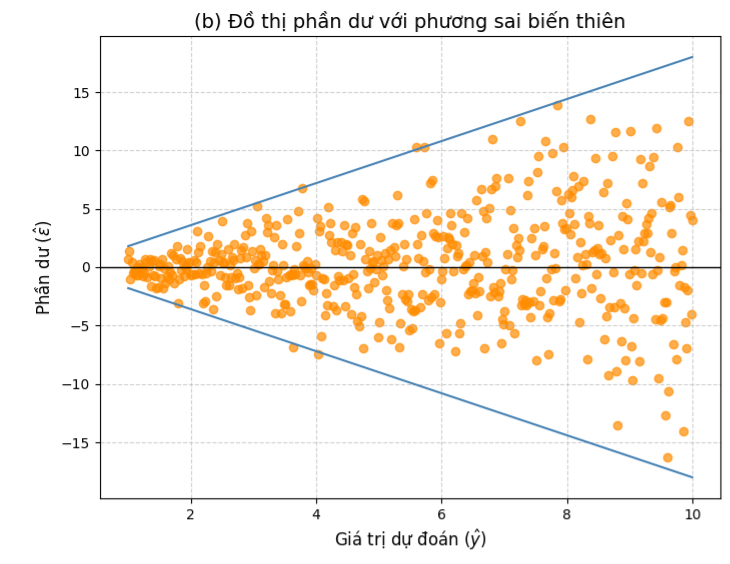
\includegraphics[width=0.9\linewidth]{images/b.png}
        \end{column}
        
        \begin{column}{0.5\textwidth}
            \textbf{Dấu hiệu tốt:}
            \begin{itemize}
                \item Phân tán ngẫu nhiên.
                \item Nằm trong một dải ngang.
            \end{itemize}
            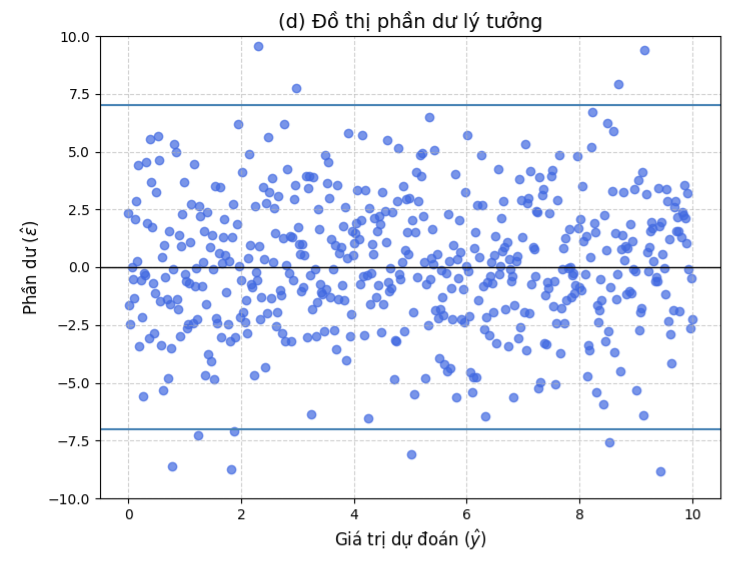
\includegraphics[width=0.9\linewidth]{images/d.png}
        \end{column}
    \end{columns}
\end{frame}

% --- Slide mới: Vẽ biểu đồ theo biến dự đoán ---
\begin{frame}
    \frametitle{Vẽ biểu đồ phần dư theo từng biến dự đoán ($X_i$)}
    \framesubtitle{Kiểm tra mối quan hệ phi tuyến bị bỏ sót}

    \begin{columns}[T] 
        \begin{column}{0.4\textwidth}
            \begin{itemize}
                \item \textbf{Hình parabol:} Bỏ sót quan hệ phi tuyến.
            \end{itemize}
            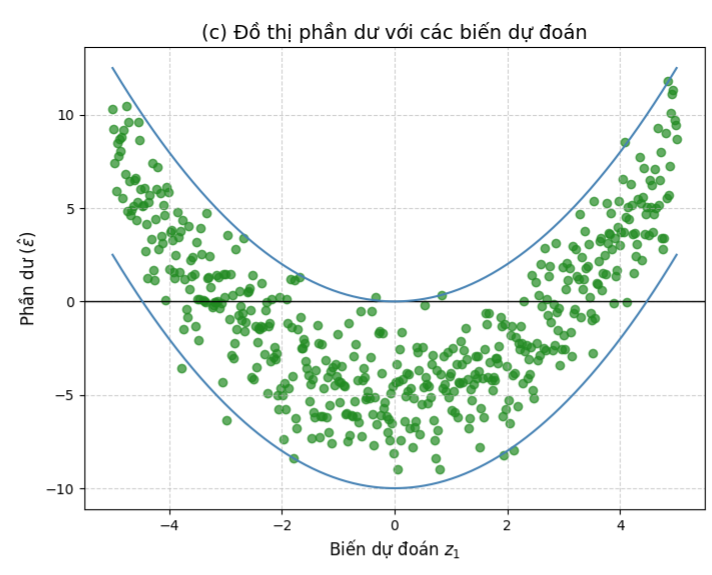
\includegraphics[width=0.9\linewidth]{images/c.png}
        \end{column}
        
        \begin{column}{0.6\textwidth}
            \begin{block}{Mục đích}
                Kiểm tra xem có một quy luật hệ thống nào giữa phần dư và một biến dự đoán \textbf{cụ thể} hay không.
            \end{block}
            
            \begin{alertblock}{Dấu hiệu vấn đề}
                Nếu biểu đồ cho thấy một quy luật có hệ thống, điều này gợi ý rằng mô hình cần có thêm các số hạng mới liên quan đến biến đó (ví dụ: $X_i^2$) để nắm bắt mối quan hệ phi tuyến.
            \end{alertblock}
        \end{column}
    \end{columns}
\end{frame}

% --- Slide Kiểm tra phân phối chuẩn ---
\begin{frame}
    \frametitle{Kiểm tra giả định phân phối chuẩn}
    \framesubtitle{Sử dụng Biểu đồ Q-Q và Histogram}
    
    \begin{block}{Tại sao quan trọng?}
        Các kiểm định t, F và khoảng tin cậy đều dựa trên giả định này. Nếu vi phạm, các giá trị p-value có thể không đáng tin cậy.
    \end{block}
    
    \begin{figure}
        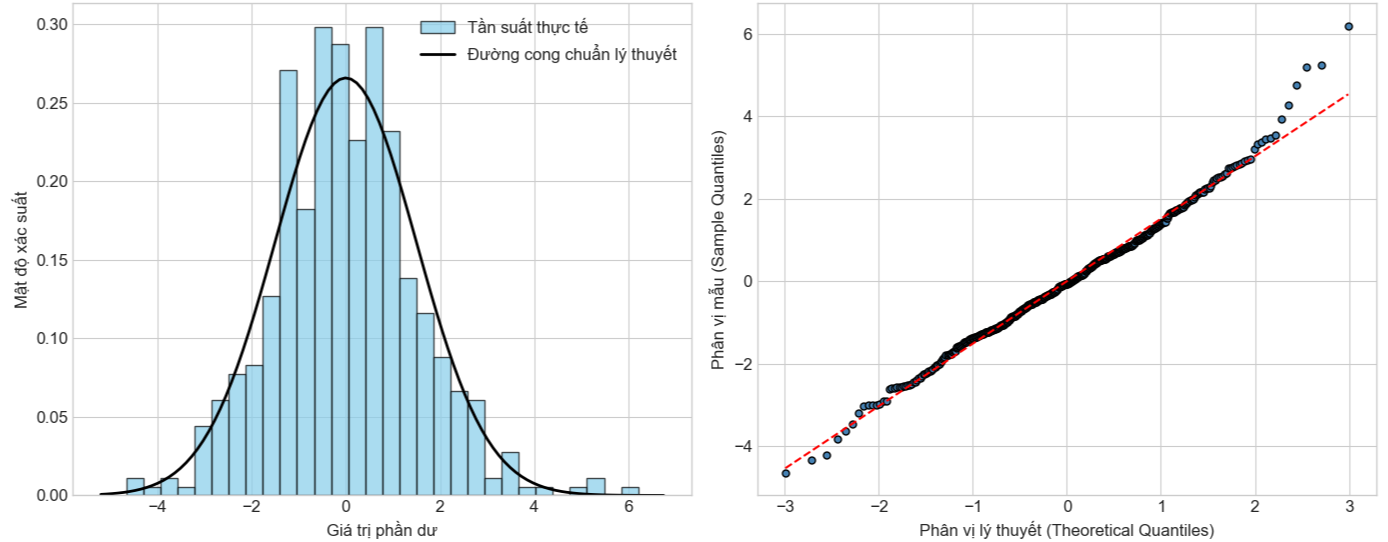
\includegraphics[width=0.7\linewidth]{images/Figure_1.png}
        \caption{Lý tưởng: Các điểm trên biểu đồ Q-Q nằm sát đường thẳng, và histogram có hình chuông.}
    \end{figure}
\end{frame}


% ===============================================================
\section{Kiểm định tính không tương quan của phần dư theo thời gian}
% ===============================================================

% --- Slide Kiểm định Tự tương quan ---
\begin{frame}
    \frametitle{Kiểm định Tự tương quan: Durbin-Watson}
    \framesubtitle{Đặc biệt quan trọng với dữ liệu chuỗi thời gian}

    Phổ biến nhất để kiểm tra tự tương quan \textbf{bậc một}, tức là mối liên hệ giữa $\varepsilon_t$ và $\varepsilon_{t-1}$.
    \begin{block}{Công thức Durbin-Watson}
        \[
        DW = \frac{\sum\limits_{t=2}^T(\widehat{\varepsilon}_t- \widehat{\varepsilon}_{t-1})^2}{\sum\limits_{t=1}^T(\widehat{\varepsilon}_t)^2} \quad \in [0, 4]
        \]
    \end{block}
    \begin{itemize}
        \item \textbf{Hạn chế:} Có "vùng không xác định" và không đáng tin cậy khi có biến trễ của Y.
    \end{itemize}
\end{frame}

\begin{frame}
    \frametitle{Kiểm định Tự tương quan: Durbin-Watson}
    \framesubtitle{Đặc biệt quan trọng với dữ liệu chuỗi thời gian}
    \textbf{Quy tắc quyết định:}
    
    Để đưa ra kết luận chính xác, cần so sánh giá trị DW với các giá trị tới hạn dL, dU từ bảng tra Durbin-Watson, dựa trên các yếu tố như mức ý nghĩa $\alpha$, cỡ mẫu n và số biến độc lập k. 
    \begin{itemize}
        \item $0 < DW < dL$ : Kết luận có tự tương quan dương.
        \item $dL \le DW \le dU$ : Không thể kết luận (vùng không xác định).
        \item $dU < DW < 4 - dU$ : Kết luận không có tự tương quan bậc nhất.
        \item $4 - dU \le DW \le 4 - dL$: Không thể kết luận.
        \item $4 - dL < DW < 4$: Kết luận có tự tương quan âm.
    \end{itemize}
\end{frame}

\begin{frame}
    \frametitle{Kiểm định Tự tương quan: Breusch-Godfrey}
    \framesubtitle{Kiểm định tổng quát cho tự tương quan bậc cao}

    Kiểm định Breusch-Godfrey (BG) là một kiểm định tổng quát và mạnh mẽ hơn DW, dùng để kiểm tra tự tương quan bậc cao.
    
    \textbf{Cách hoạt động:} Chạy một hồi quy phụ của phần dư theo các biến độc lập ban đầu và các phần dư trễ ($\varepsilon_{t-1},...,\varepsilon_{t-p})$.
    
    \begin{block}{Mô hình hồi quy phụ}
    \setlength{\abovedisplayskip}{0pt}
        \[
        \widehat{\varepsilon}_t = \alpha_0 + \beta_1 X_{1,t} + \ldots + \beta_k X_{k,t} + \alpha_1 \widehat{\varepsilon}_{t-1} + \alpha_2 \widehat{\varepsilon}_{t-2} + \ldots + \alpha_p \widehat{\varepsilon}_{t-p} + u_t
        \]
    \end{block}
    
    \begin{itemize}
        \item \textbf{Giả thuyết:} $H_0: \alpha_1 = \alpha_2 = \ldots = \alpha_p = 0$ (Không có tự tương quan đến bậc $p$).
        \item \textbf{Thống kê kiểm định:} $LM = nR^2 \sim \chi^2(p)$
        \item \textbf{Quyết định:} Nếu $p$-value của thống kê $LM$ là nhỏ ($< 0.05$), ta bác bỏ $H_0$ và kết luận có tồn tại tự tương quan.
    \end{itemize}
\end{frame}


% ===============================================================
\section{Xác định các biến quan trọng}
% ===============================================================

% --- Slide Tổng quan ---
\begin{frame}
    \frametitle{Xác định các biến quan trọng}
    \framesubtitle{Tại sao cần lựa chọn biến?}
    Vấn đề với mô hình có quá nhiều biến:
    \begin{itemize}
        \item \textbf{Overfitting:} Mô hình fit tốt trên train ($R^2$ cao) nhưng dự đoán kém trên test
        \item \textbf{Đa cộng tuyến:} Các hệ số không ổn định, phương sai lớn và p-value không đáng tin cậy.
        \item \textbf{Khó diễn giải:} Quá nhiều biến làm mô hình phức tạp
        \item \textbf{Chi phí thu thập dữ liệu:} Thực tế không cần thiết
    \end{itemize}
    \textbf{Mục tiêu:} Tìm tập con biến nhỏ nhất nhưng vẫn giải thích tốt biến phụ thuộc.
        
    \textit{"As simple as possible, but not simpler"} - Einstein
\end{frame}

% --- Slide Các phương pháp lựa chọn biến ---
\begin{frame}
    \frametitle{Các tiêu chí đánh giá mô hình}
    \framesubtitle{Hồi quy từng bước (Stepwise Regression)}
    Một thuật toán tự động để thêm/bớt các biến dựa trên một tiêu chí thống kê (ví dụ: F-test, p-value).
    
    \textbf{Lựa chọn tiến (Forward Selection):}
    \begin{enumerate}
        \item Bắt đầu với mô hình rỗng (chỉ có hệ số chặn).
        \item Lần lượt thêm từng biến vào và chọn biến có p-value thấp nhất (và < $\alpha$).
        \item Lặp lại cho đến khi không còn biến nào có thể thêm vào.
    \end{enumerate}
\end{frame}

\begin{frame}
    \frametitle{Các tiêu chí đánh giá mô hình}
    \framesubtitle{Hồi quy từng bước (Stepwise Regression)}

    \textbf{Loại bỏ lùi (Backward Elimination):}
    \begin{enumerate}
        \item Bắt đầu với mô hình đầy đủ (chứa tất cả các biến).
        \item Tìm biến có p-value cao nhất và lớn hơn ngưỡng $\alpha$ (thường là 0.05).
        \item \textbf{Loại bỏ} duy nhất biến đó.
        \item Chạy lại mô hình với các biến còn lại.
        \item Lặp lại quy trình cho đến khi tất cả các biến trong mô hình đều có p-value nhỏ hơn $\alpha$.
    \end{enumerate}
\end{frame}

\begin{frame}
    \frametitle{Các tiêu chí đánh giá mô hình}
    \framesubtitle{Hồi quy từng bước (Stepwise Regression)}
    
    \textbf{Chọn hỗn hợp (Mixed Selection):}
    \begin{itemize}
        \item Đây là phương pháp kết hợp cả Forward và Backward.
        \item Sau mỗi bước thêm vào một biến mới, thuật toán sẽ kiểm tra lại tất cả các biến đã có trong mô hình.
        \item Nếu có biến nào trở nên không còn ý nghĩa (ví dụ p-value > $\alpha$), biến đó sẽ bị loại ra.
        \item Quá trình dừng lại khi không thể thêm vào hay loại ra bất kỳ biến nào nữa.
    \end{itemize}
\end{frame}

\begin{frame}
    \frametitle{Các tiêu chí đánh giá mô hình}
    \framesubtitle{Hệ số xác định $R^2$ hiệu chỉnh}
    Hệ số xác định $R^2$:
    \[
    R^2 = 1 - \frac{RSS}{TSS} 
    \]
    $R^2$ hiệu chỉnh:
    \[
    R^2_{adj} = 1 - \frac{RSS}{TSS}.\frac{n-1}{n-p-1}
    \]
    \begin{itemize}
        \item $R^2$: Luôn tăng khi thêm biến (kể cả biến vô dụng)
        \item $R^2_{adj}$: Có thể giảm nếu biến thêm vào không đủ tốt
        \item \textbf{Quy tắc:} Chọn mô hình có $R^2_{adj}$ cao nhất
    \end{itemize}
\end{frame}

\begin{frame}
    \frametitle{Các tiêu chí đánh giá mô hình}
    \framesubtitle{Mallow's Cp}
    So sánh mô hình con với mô hình đầy đủ. Mô hình tốt sẽ có giá trị $C_p$ nhỏ và xấp xỉ số tham số ($p+1$).
    \[C_p = \frac{RSS_p}{\widehat{\sigma}^2} - n + 2(p+1)\]
    \begin{enumerate}
        \item Tính $C_p$ cho tất cả các mô hình con
        \item Vẽ đồ thị $C_p$ vs. $p+1$
        \item Chọn mô hình có $C_p$ \textbf{nhỏ} và các điểm $(p+1,C_p)$ nằm gần đường chéo $45^{\circ}$
    \end{enumerate}
\end{frame}

\begin{frame}
    \frametitle{Các tiêu chí đánh giá mô hình}
    \framesubtitle{AIC (Akaike's Information Criterion)}
    Mô hình có AIC nhỏ hơn thì tốt hơn.
    \[ AIC = n \ln(\frac{RSS_p}{n}) + 2(p+1) \]
    \textbf{Ưu điểm}
    \begin{itemize}
        \item Có xu hướng chọn mô hình tốt nhất để tối ưu hóa khả năng dự đoán 
        \item Thường hoạt động tốt với mẫu nhỏ
    \end{itemize}
    
    \textbf{Nhược điểm}
    \begin{itemize}
        \item Khi cỡ mẫu $n$ rất lớn, AIC vẫn có xác suất chọn phải mô hình quá phức tạp (overfitting) và không hội tụ về "mô hình thật" (true model).
    \end{itemize}
\end{frame}
\begin{frame}
    \frametitle{Các tiêu chí đánh giá mô hình}
    \framesubtitle{BIC (Bayesian Information Criterion)}
    Tương tự AIC nhưng phạt nặng hơn khi thêm biến (với n lớn)
    \[ BIC = n \ln\left(\frac{RSS_p}{n}\right) + (p+1)\ln(n) \]
    
    \textbf{Ưu điểm}
    \begin{itemize}
        \item Ưu tiên sự đơn giản: Mức phạt $\ln(n)$ rất nặng, giúp tránh overfitting hiệu quả trong các bộ dữ liệu lớn.
        \item Khi $n$ đủ lớn, BIC có khả năng tìm ra "mô hình thật" với xác suất cao (tốt cho mục tiêu giải thích).
    \end{itemize}
    
    \textbf{Nhược điểm}
    \begin{itemize}
        \item Không phù hợp với các bộ dữ liệu mẫu nhỏ, có xu hướng chọn mô hình quá đơn giản (under-fitting).
    \end{itemize}
\end{frame}


\begin{frame}
    \frametitle{So sánh các phương pháp lựa chọn biến}
    
    \begin{table}
    \centering
    \scriptsize
    \begin{tabular}{|l|c|c|l|}
    \hline
    \textbf{Phương pháp} & \textbf{Mục tiêu} & \textbf{Tốc độ} & \textbf{Ghi chú} \\
    \hline
    Stepwise & Minimize AIC / RSS & Trung bình & Tự động thêm hoặc loại biến \\
    \hline
    $R^2_{adj}$ & Maximize & Nhanh & Đơn giản, dễ so sánh mô hình \\
    \hline
    AIC & Minimize & Nhanh & Ưu tiên độ phù hợp (fit) \\
    \hline
    BIC & Minimize & Nhanh & Ưu tiên mô hình đơn giản \\
    \hline
    $C_p$ (Mallows) & $\approx p+1$ & Trung bình & Liên quan chặt chẽ với AIC \\
    \hline
    \end{tabular}
    \end{table}
\end{frame}


% ===============================================================
\section{Các bước thiết lập mô hình hồi quy tuyến tính}
% ===============================================================

% --- Slide Quy trình ---
\begin{frame}
    \frametitle{Quy trình 5 bước xây dựng mô hình hồi quy}
    \begin{enumerate}
        \item \textbf{Khám phá và Chuẩn bị dữ liệu (EDA):}
        \begin{itemize}
            \item Trực quan hóa, xử lý dữ liệu thiếu, kiểm tra đa cộng tuyến.
            \item Chia tập Train/Test ngay từ đầu
        \end{itemize}

        \item \textbf{Lựa chọn biến và Xây dựng mô hình (Trên tập Train):}
        \begin{itemize}
            \item Sử dụng Stepwise, p-value, AIC, Adjusted $R^2$, $C_p$ để chọn mô hình ứng viên.
        \end{itemize}

        \item \textbf{Chẩn đoán và Tinh chỉnh mô hình (Trên tập Train):}
        \begin{itemize}
            \item Kiểm tra giả định thông qua phần dư (tuyến tính, phương sai, chuẩn, độc lập).
            \item Phân tích outlier. Nếu vi phạm, quay lại Bước 2.
        \end{itemize}

        \item \textbf{Đánh giá hiệu năng cuối cùng (Trên tập Test):}
        \begin{itemize}
            \item Dùng mô hình cuối cùng để dự đoán trên tập test.
            \item Tính các chỉ số lỗi: MAPE, RMSE, MAE.
        \end{itemize}
        
        \item \textbf{Diễn giải và Báo cáo:}
        \begin{itemize}
            \item Trình bày phương trình, ý nghĩa hệ số và các kết quả đánh giá.
        \end{itemize}
    \end{enumerate}
\end{frame}